\documentclass{article}
\usepackage{enumitem}
\usepackage{amsmath, amsthm, amssymb, esint, mathtools}

%Geometry
\usepackage[a4paper,lmargin=1.2in,rmargin=1.2in,bmargin=1.5in]{geometry}

%Header and Footer
\usepackage{fancyhdr}
\pagestyle{fancy}
\fancyhf{}
\lhead{190050034-190050097}
\cfoot{Page \thepage}
\renewcommand{\headrulewidth}{0.4pt}
\renewcommand{\footrulewidth}{0.4pt}
\addtolength{\skip\footins}{2pc plus 5pt}

%Links
\usepackage{enumitem}
\usepackage{hyperref}
\usepackage{float}
\usepackage{graphicx}
\usepackage{subfig}

%Theorems
\newtheorem{prp}{Proposition}
\theoremstyle{remark}
\newtheorem*{remark}{Remark}

%Other settings
\setlength{\parindent}{0pt}

%Macros
\newcommand{\bN}{\mathbb{N}}
\newcommand{\bR}{\mathbb{R}}
\newcommand{\bC}{\mathbb{C}}
\newcommand{\dsp}[1]{\displaystyle{#1}}
\newcommand{\Intersect}[2]{\overset{#2}{\underset{#1}{\wedge}}}
\newcommand{\bs}[1]{\boldsymbol{#1}}
\newcommand{\inner}[2]{\langle #1,#2 \rangle}
\newcommand{\ltwo}[1]{||#1||_{2}}
\newcommand{\lone}[1]{||#1||_{1}}
\newcommand{\lstar}[1]{||#1||_*}
\newcommand{\lfro}[1]{||#1||_F}
\newcommand{\lnorm}[1]{\left\lVert#1\right\rVert}
\newcommand{\norm}[1]{\left\lVert#1\right\rVert}
\DeclareMathOperator*{\argmax}{arg\,max}
\DeclareMathOperator*{\argmin}{arg\,min}

\title{Project Report}
\author{190050034-190050097}

\begin{document}
\hypersetup{pageanchor=false}
\maketitle
\pagenumbering{arabic}

The project is aimed to study the paper :
\begin{center}
Approximation and Compression using Sparse Orthogonal Transform\\
by\\
Osman G. Sezer, Onur G. Guleryuz and Yucel Altunbasak
\end{center}
which aims at constructing a \textbf{data driven Orthogonal Transform} which extends over the Karhunen-Loeve Transform which is known to be optimal on Gaussian Processes. For gaussian processes, this method reduces to the KLT, and performs siginificantly better on other processes.

\section*{KLT is equivalent to SOT on Gaussian Processes}
The major theoretical point made in the paper is this. The definition of SOT is in terms of solution to a minimization problem given by :
$$SOT = argmin_{G}[ E( min_\alpha \{||x-G\alpha||_2^2 + \lambda||\alpha||_0\} ) ] \backepsilon GG^T = G^TG = I$$
\begin{prp}
Let $x$ be a zero mean random variable $(\bR^n)$ with covariance matrix $\Sigma$. Given any function $W$ over orthonormal matrices $(\in \bR^{n\times n})$ of the form
$$W(G) = \sum_{i=1}^n f(g_i^T \Sigma g_i)$$
where $f$ is a concave function. The matrix $P$ of eigenvectors of $\Sigma$ is a minimizer of $W$.
\end{prp}
\begin{proof}
Let $G$ be arbitrary. It is clear that $\Sigma = P\Lambda P^T$ for a diagonal matrix $\Lambda$. Let $R = P^TG$ be another orthogonal matrix. Then,
$$ f(g_i^T\Sigma g_i) = f(g_i^T P \Lambda P^T g_i) = f(r_i^T \Lambda r_i) = f(\sum_{j=1}^n r_{i,j}^2 \lambda_{jj})$$
Since, $f$ is concave and $\sum_{j=1}^n r_{i,j}^2 = 1$, using Jensen's inequality it is clear that
$$f(g_i^T\Sigma g_i) f(\sum_{j=1}^n r_{i,j}^2 \lambda_{jj}) \geq \sum_{j=1}^n r_{i,j}^2 f(\lambda_{jj}) = r_i^T Q r_i = g_i^T PQP^T g_i$$
where $Q$ is a diagonal matrix with entries $Q_{ii} = f(\lambda_{ii})$. Thus,
$$\sum_{i=1}^n f(g_i^T\Sigma g_i) \geq \sum_{i=1}^n g_i^T PQP^T g_i = Tr[G^TPQP^TG]$$
Using the identity $Tr[AB] = Tr[BA]$, we obtain
$$Tr[G^TPQP^TG] = Tr[GG^TPQP^T] = Tr[PQP^T] = Tr[P^TPQ] = Tr[Q] = \sum_{i=1}^n f(\lambda_{ii})$$
Furher, notice that $W(P) = \sum_{i=1}^n f(g_i^T \Sigma g_i) = \sum_{i=1}^n f(p_i^T P \Lambda P^T p_i) = \sum_{i=1}^n f(\lambda_{ii})$
\end{proof}
First we would like to know how to solve for $\alpha$, given $x$ and $G$. The solution turns out to be a simple thresholding of the solution to $x = G\alpha$.
\begin{prp}
The vector $c$ defined by
$$c_i = \begin{cases}
	g_i^T x & |g_i^T x| \geq \sqrt{\lambda}\\
	0 & \text{otherwise}
\end{cases}$$
is the solution to $argmin_\alpha (||x - G\alpha||_2^2 + \lambda||\alpha||_0)$.
\end{prp}
\begin{proof}
$$||x-G\alpha||_2^2 = ||G^Tx - G^TG\alpha||_2^2 = ||G^Tx - \alpha||_2^2$$
since $G$ is orthonormal. Furthermore,
$$||x - G\alpha||_2^2 + \lambda||\alpha||_0 = ||G^Tx - \alpha||_2^2 + \lambda||\alpha||_0 = \sum_{i=1}^n |g_i^Tx - \alpha_i|^2 + \lambda I(\alpha_i \neq 0)$$
The minimization can be carried out for each $\alpha_i$ independently and results in the thresholding.
\end{proof} 

Using the ideas in propositions 1 and 2, we observe that:
$$E(min_\alpha \{||x-G\alpha||_2^2 + \lambda||\alpha||_0\}) = E(\sum_{i=1}^n min_{\alpha_i} \{ |g_i^Tx - \alpha_i|^2 + \lambda I(\alpha_i \neq 0)\})$$
Since sum distributes over expectations, we obtain
$$E(min_\alpha \{||x-G\alpha||_2^2 + \lambda||\alpha||_0\}) = \sum_{i=1}^n E( min_{\alpha_i} \{ |g_i^Tx - \alpha_i|^2 + \lambda I(\alpha_i \neq 0)\})$$
If $x$ is a zero mean gaussian random variable with covariance matrix $\Sigma$, $g_i^Tx$ is a scalar gaussian random variable with variance $g_i^T\Sigma g_i$. Using this fact, an individual expectation can be evaluated.
$$E( min_{\alpha_i} \{ |g_i^Tx - \alpha_i|^2 + \lambda I(\alpha_i \neq 0)\} ) \propto \int_0^{\sqrt{\lambda}} y e^{-y^2/2\sigma_i^2} dy + \lambda \int_{\sqrt{\lambda}}^{\infty} e^{-y^2/2\sigma_i^2}dy$$
where $\sigma_i^2 = g_i^T \Sigma g_i$. Thus, the expectation can be written as a function $f(g_i^T\Sigma g_i)$, and the objective function for SOT as a sum of form
$$\sum_{i=1}^n f(g_i^T\Sigma g_i)$$
It can be checked that $f$ is a concave function as its second order derivative is always negative. Using proposition 1, $P$ is a minimizer of the objective function and thus SOT is equivalent to KLT on a zero mean Gaussian process.
\newpage

\section*{Finding the SOT}
\subsection*{Algorithm}
Finding the SOT for a sample of vectors $X$ for given $\lambda$ works via a 2 step minimizaton:\\[1mm]
A random initial transform $H$ is chosen. Then, until convergence,
\begin{enumerate}
\item Evaluate the best coefficients (constant transform)
\item Evaluate the best transforms (constant coefficients)
\end{enumerate}
Which is the general trend of dictionary learning algorithms.\\[2mm]
Proposition 2 stated how we can perform step 1. Step 2 is demonstrated :\\[1mm]
Since the coefficents are set to be constant, we need to minimize 
$$E( ||x - G\alpha||_2^2)$$
We do not have knowledge of the distribution on $x$. All we have is a dataset $X$ consisting of a large number of samples. We instead minimize the data driven expected value
$$\hat{E} (||x-G\alpha||_2^2) = ||X - GA||_F^2$$
for an orthogonal matrix $G$. This is an orthogonal procrustes problem.\\[1mm]
Efficient solution of the problem is known and is given by
$$UV^T \text{ where } AX^T = U\Sigma V^T \text{ with orthonormal } U,V \text{ and diagonal } \Sigma$$
We expect to use this algorithm with a few additions (classification and annealing) to beat the KLT on image datasets in terms of compression properties.\\[1mm]
For the initial transform provided as an input, we use the KLT.
\subsection*{Peculiarities of the Algorithm}
We list a few points we find interesting about the algorithm.\\[1mm]
The algorithm is similar to overcomplete dictionary learning using a collection of orthonormal dictionaries but it is different in the sense that reconstruction follows by chosing the best basis.\\
This guarentees that reconstructions would be faster (as we do not solve a complex optimization problem) and unique irrespective of conditions needed in overcomplete dictionary learning.
\subsection*{Drawbacks of the Algorithm}
We list a few drawbacks we find in the algorithm.\\[2mm]
The algorithm does not function well for low and high values of $\lambda$. For low values, we do not observe much change in direction. For high values, accuracy is compromised significantly. Thus, hyper-parameter tuning is a concern.\\[1mm]
Further, it is a convergence based algorithm and even though convergence is theoretically guarenteed, it will remain slow compared to KLT, which is a one step transformation. Reclassification and Annealing only slow the process further.
\newpage

\section*{SOT vs KLT Results on Synthetic Test Data}

\subsection*{Gaussian Noise}
\begin{figure}[H]
\centering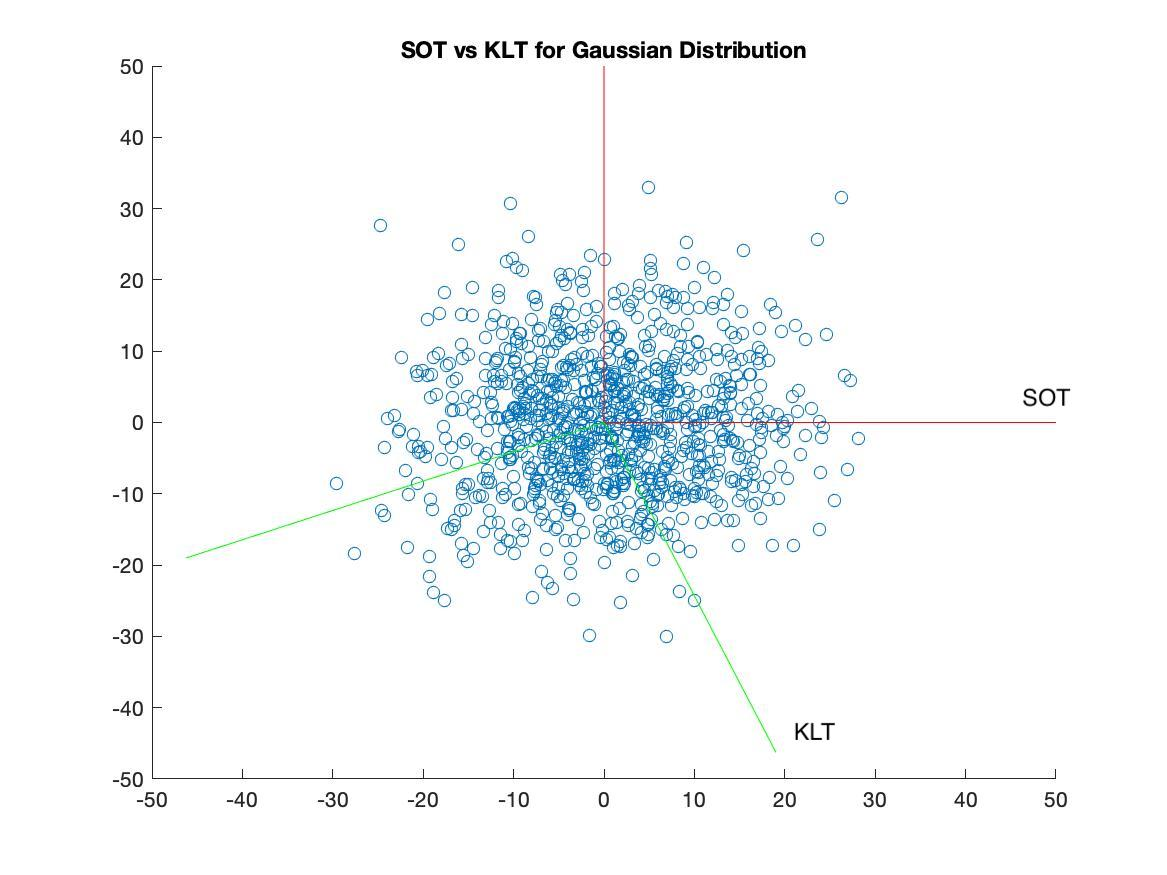
\includegraphics[width=0.6\linewidth]{images/gaussian.jpg}
\caption{KLT and SOT Matrices for Gaussian Distribution $\mathcal{N}(100I)$}
\end{figure}
As can be seen, the SOT and KLT both produce optimal directions.
\subsection*{Non Gaussian Noise}
\begin{figure}[H]
\centering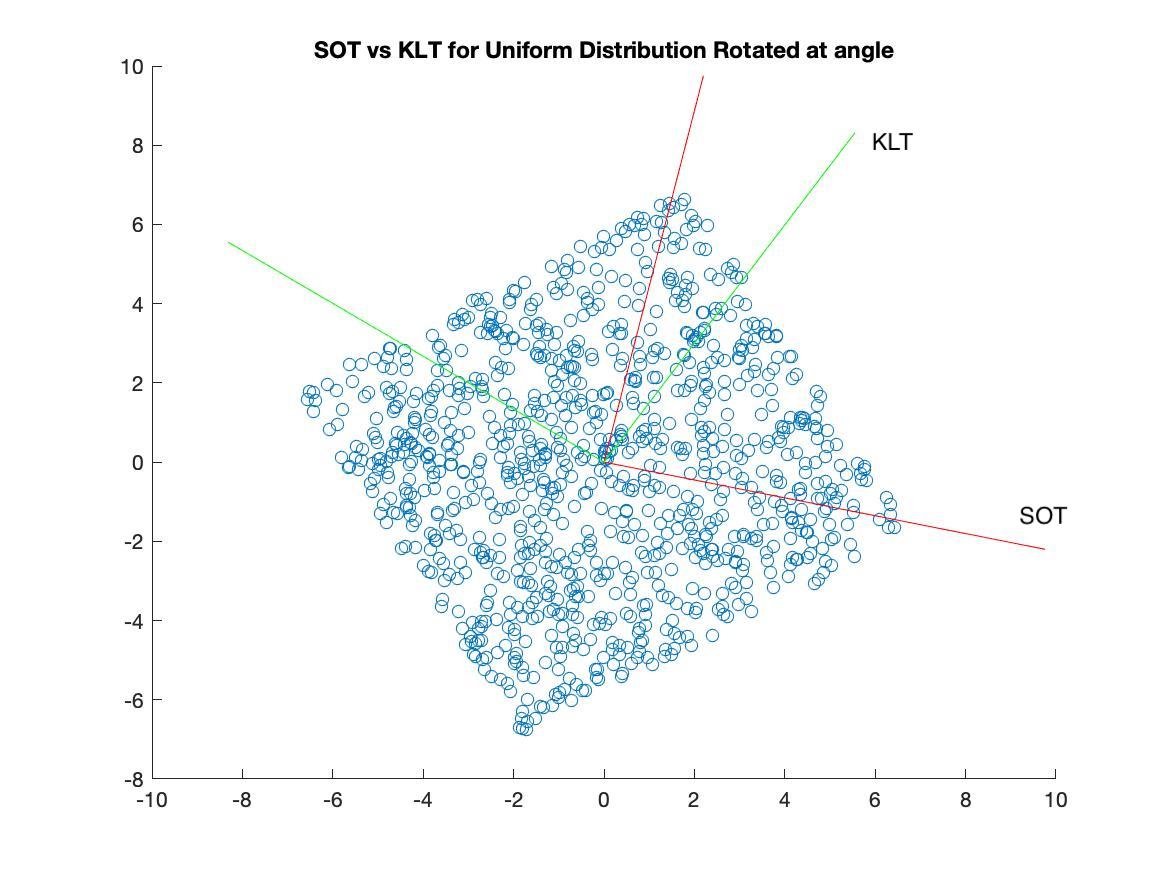
\includegraphics[width=0.6\linewidth]{images/uniform.jpg}
\caption{KLT and SOT Matrices for Uniform Distribution rotated by $30^\circ$ ACW}
\end{figure}
\begin{figure}[H]
\centering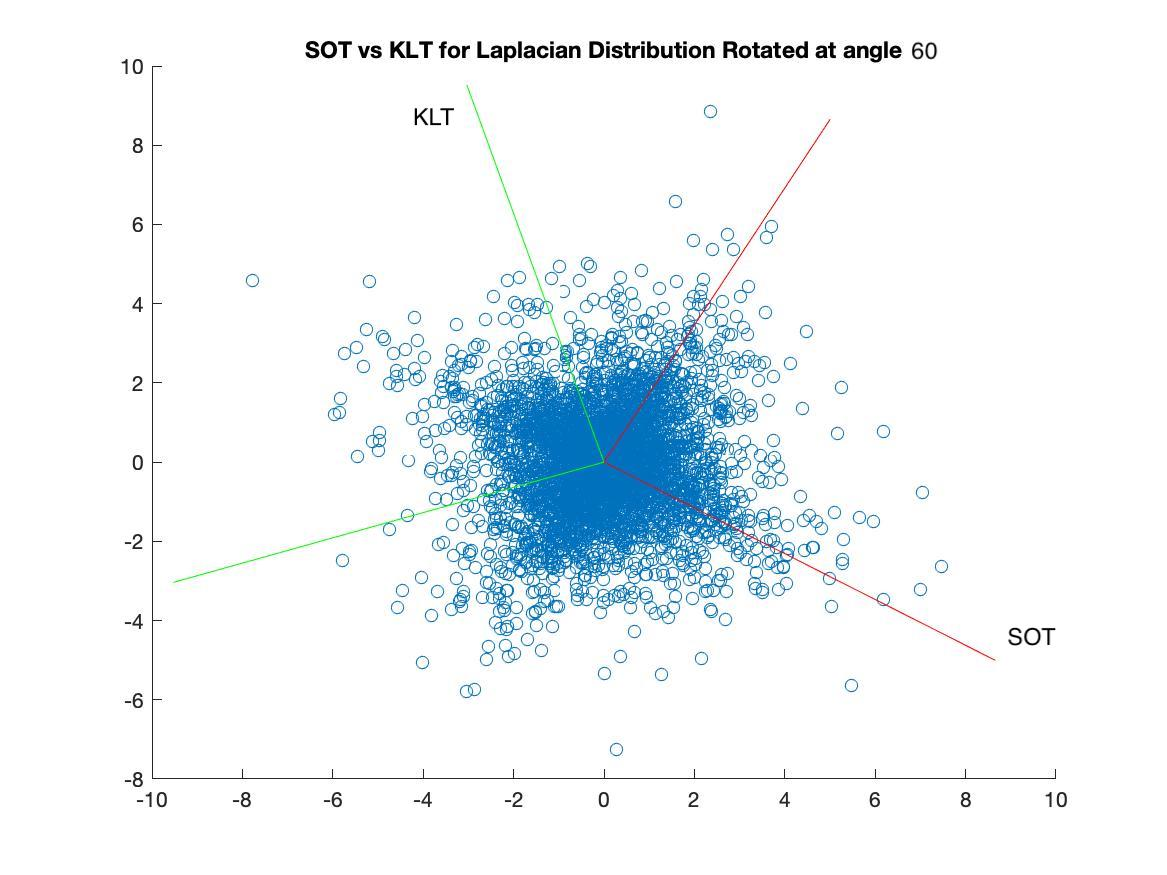
\includegraphics[width=0.6\linewidth]{images/laplacian.jpg}
\caption{KLT and SOT Matrices for Laplacian Distribution rotated by $60^\circ$ ACW}
\end{figure}
In both these cases, we observe that SOT finds a direction where coefficients are expected to be sparser compared to the KLT. In the case of uniform noise, the KLT is degenerate and any orthogonal basis serves as KLT.\\[2mm]
This guarentee the initial claim, which is, the SOT and KLT are equivalent on zero mean Gaussian processes whereas the SOT has the capability to outperform KLT on other processes.
\subsection*{Tabulated Results}
The NL-cost and relative cost error between the 2 methods is as mentioned in table
\begin{table}[H]
\centering
\begin{tabular}{| c | c | c | c |}
\hline
\textbf{Distribution} & \textbf{SOT Cost} & \textbf{KLT Cost} & \textbf{Rel. Cost}\\
\hline
Gaussian & 1.8900e+03 & 1.8866e+03 & 0.0018\\
Uniform & 1.6591e+03 & 1.6986e+03 & 0.0232\\
Laplacian & 5.2907e+03 & 5.7982e+03 & 0.0875\\
\hline
\end{tabular}
\end{table}

Hence we can see we get a big difference for non gaussian data between SOT and KLT distributions.

\newpage
\section*{SOT vs KLT vs DCT on Image Compression}
\subsection*{The Experiment}
\subsubsection*{Data}
A dataset of $8\times 8$ patches obtained from the first 20 images available in {\tt code/data/} folder. The data is obtained from \href{http://sipi.usc.edu/database/database.php?volume=misc}{here} and each image is converted to greyscale using standard conversion procedures in openCV.
\subsubsection*{Validation}
Since hyperparameter tuning was a concern, we used a range of values of $\lambda$ and kept $\delta = \lambda$ and $\lambda_{max} = 10\lambda$ for convenience. We trained dictionaries using only 5 of the 20 images obtained with different values of $\lambda$.\\[1mm]
For every image in the validation set, i.e. images 31-33 in the folder {\tt code/data/}, we perform a non-overlapping patchwise reconstruction using these bases. Only the largest $n$ values (in absolute value sense) are kept in each patch and reconstruction is performed using them. We then plot PSNR between the original image and the reconstructions vs $n$.\\[1mm]
All the plots obtained were of the following form :
%% Add the image with proper labelling
In the rather cluttered plot, the following observations can be made :
\begin{enumerate}
\item For very low values of $\lambda$, the PSNR is low throughout. This is because for extremely small values of $\lambda$, the cost function for SOT reduces to the squared norm difference between the image and its reconstruction, which, the KLT is known to minimize. Thus, we do not obtain the benefits we expected by using SOT over KLT.
\item For very high values of $\lambda$, the PSNR starts off high but drops down significantly as $n$ increases. The straightforward explaination is a high value of $\lambda$ promotes sparsity above reconstruction accuracy.
\end{enumerate}
We observe that the plots corresponding to $\lambda \in \{ 1e-3, 2e-3\}$ perform well on a large range of $n$ values. We thus set $\lambda = 2e-3$ for training the final dictionary. The code for this part can be obtained in {\tt code/validation/} directory along with the learnt bases and more plots.
\subsubsection*{Final Training}
A KLT basis is obtained and a group of $K=8$ SOT bases are obtained by offline training on the complete 20 image dataset. The code can be obtained in {\tt code/finaltraining/} folder.\\[1mm]
Note : The basis learning process is time consuming (we needed 15 minutes on a state of the art system) and hence we have saved the matlab variables in a file {\tt code/dict.mat}. We use this for demonstration purposes as the algorithm is deterministic.
\subsubsection*{Testing}
Testing was done on 10 images (21-30 from the dataset). For each image in the test set, reconstructions were obtained using the learng SOT, KLT and DCT bases keeping only the top $n$ entries. PSNR vs $n$ plots were obtained.
\subsection*{Results}
Consider the following reconstructions obtained using SOT, KLT and DCT keeping only $n = 10$ coefficients in a batch. SOT significantly outperforms DCT and has a better reconstruction than KLT.
%% Add the image in a 2x2 grid with appropriate subcaptions. Use the airplane image.
A few plots obtained in testing follow :
\begin{figure}
\centering
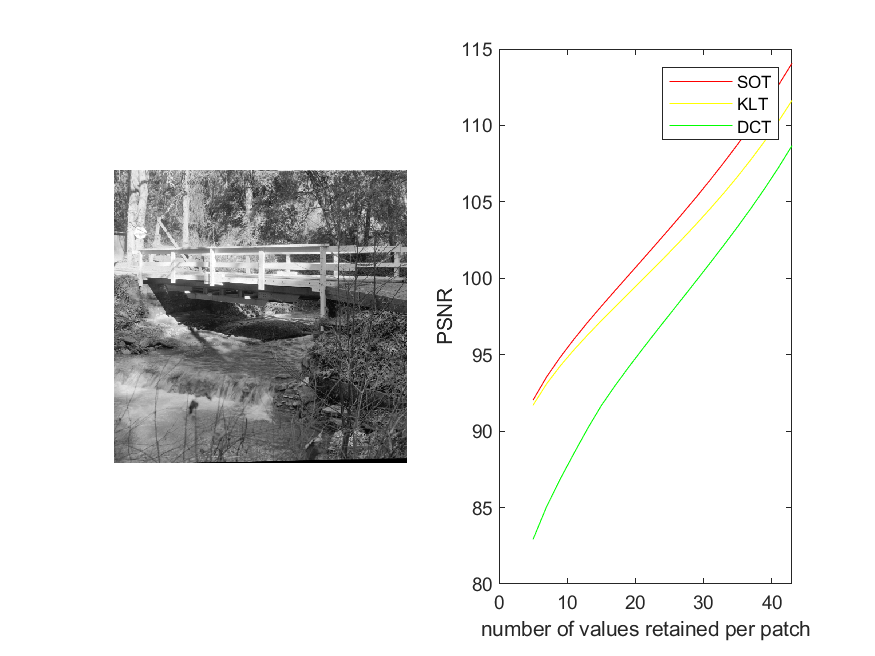
\includegraphics[width=0.9\linewidth]{images/test1.png}
\caption{SOT vs DCT vs KLT demonstration 1}
\end{figure}
\begin{figure}
\centering
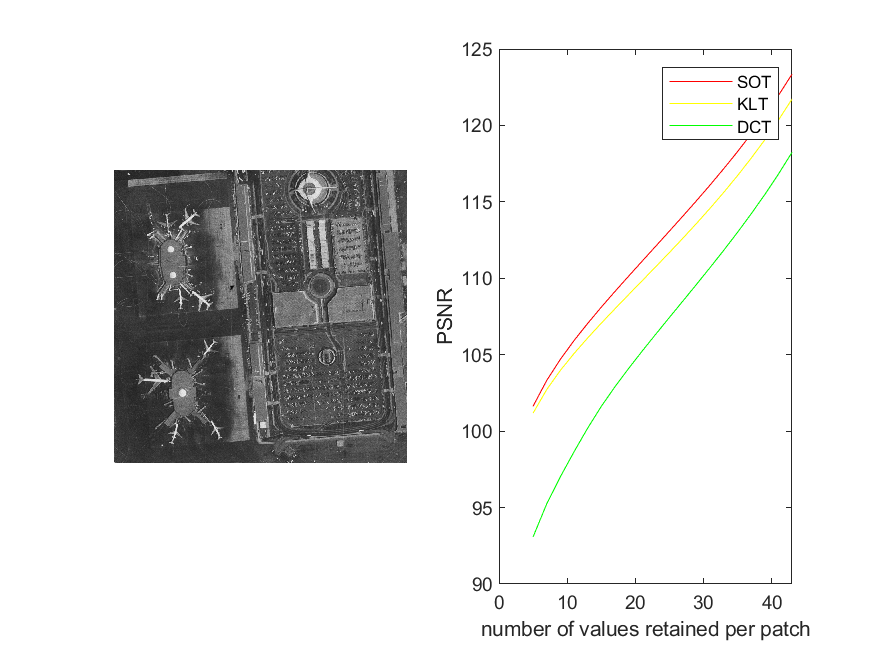
\includegraphics[width=0.9\linewidth]{images/test2.png}
\caption{SOT vs DCT vs KLT demonstration 1}
\end{figure}
\begin{figure}
\centering
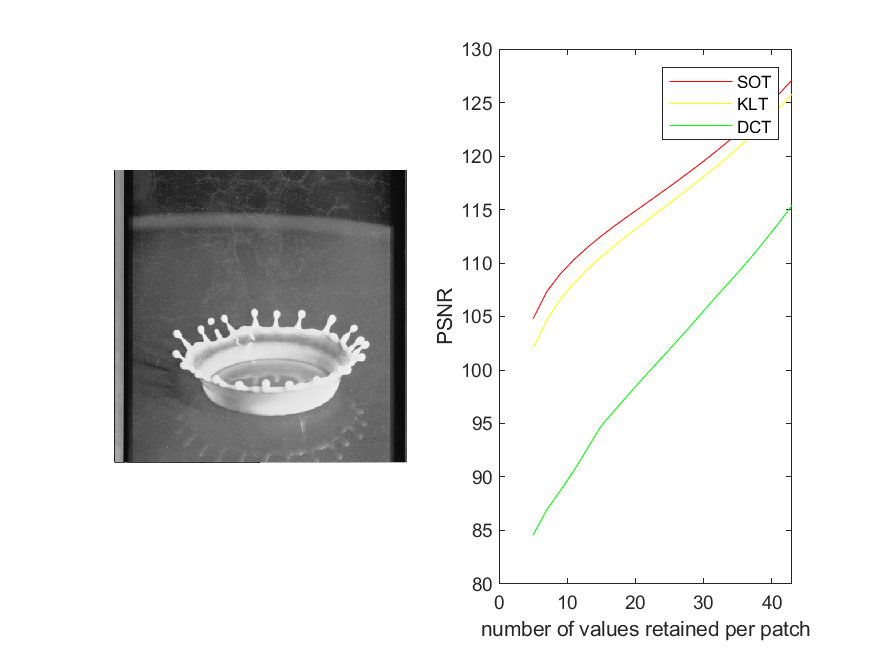
\includegraphics[width=0.9\linewidth]{images/test3.png}
\caption{SOT vs DCT vs KLT demonstration 1}
\end{figure}
It can be seen that at vert low values of $n$, SOT and KLT behave similarly but for interesting ranges of $n$ (between 15-35), SOT outperforms KLT. DCT starts off very poor but quickly picks up coming closer to KLT, DCT in the values of $n \approx 20-40$, justifying the popularity of the JPEG compression algorithm.\\[1mm]
We observe that using a good value of $\lambda$, SOT can provide significant benefits over KLT which is what we sought after.\\[1mm]
The code and more results can be obtained in {\tt code/testing/} folder.
\subsubsection*{Comments}
The following improvements can be made to the experiment :
\begin{enumerate}
\item The use of quad-tree based implementation mentioned in the paper. We expect a slight improvement in border pecularities.
\item Use of adaptive patch sizes along with the Quad Tree based implementation. The paper states a significant improvement in PSNR on using this method.
\item Using the SOT in Wavelet basis might improve performance and is mentioned as a specialization in the paper.
\item Better hyperparameter tuning ($\lambda, \lambda_{max}, \delta, \epsilon$) with a larger validation set can be performed.
\end{enumerate}
\end{document}